\section{Project: Icarus Overview}
\label{sec:overview}

Project: Icarus incorporates a novel airframe design paired with a highly
custom flight computer stack that blends together the hardware advantages of
fixed wing aircraft and multirotor aircraft in a hybrid-VTOL aircraft with the
capability to transition  between multirotor and fixed wing flight. The
airframe is constructed using carbon  fibre and is designed to be lightweight
and durable.

Characteristics of the Project: Icarus airframe include a wingspan of 2.4 m and
a wing chord length of 0.4 m. The horizontal stabilizers have a span of 0.8 m,
chord length of 0.32 m, and the two vertical stabilizers, one attached at each
end of the horizontal stabilizer, are 0.3 m tall. The booms are 1.2 m long.

\begin{figure}[ht]
        \centering
        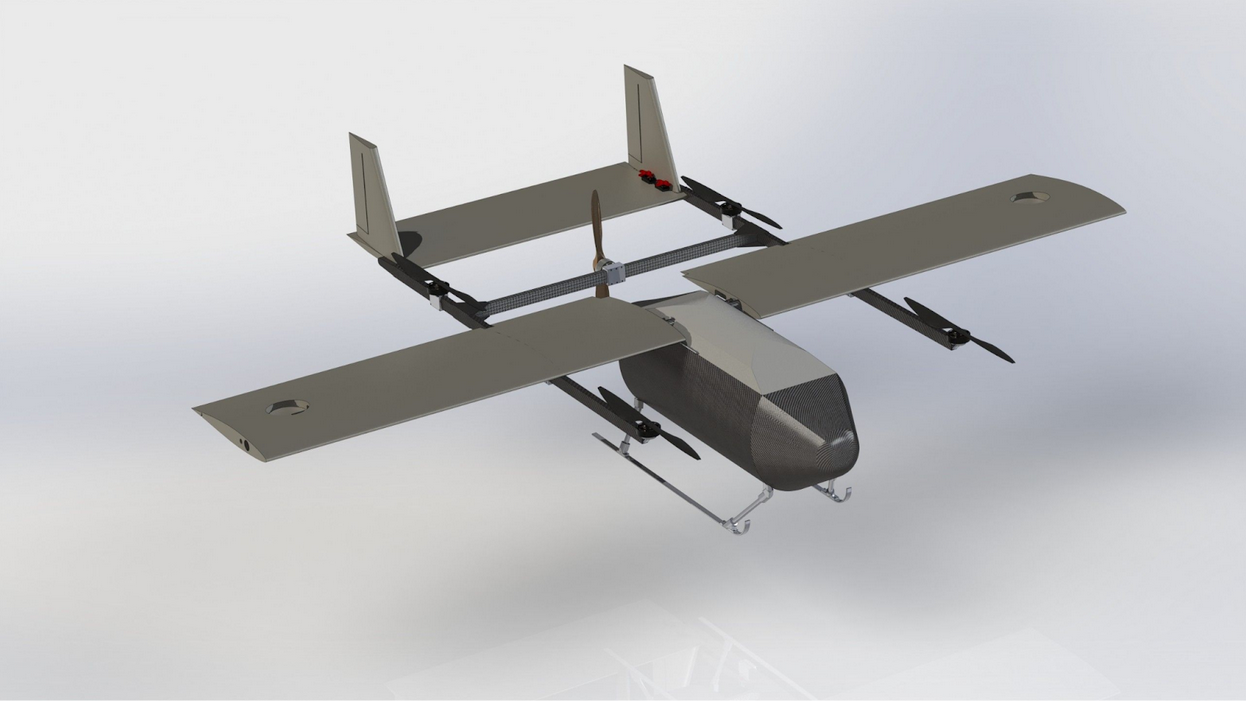
\includegraphics[scale=0.5]{frame}
        \caption{Project: Icarus airframe CAD render}
\end{figure}

In terms of materials, the structural H-shaped frame of the aircraft, which
includes the two booms the rear cross-beam, the fuselage, and supports are
constructed using carbon fibre and a combination of twill tubing and sheets.
The wings and tail are made from CNC-cut XPS foam. The NACA 64A210 airfoil was
chosen for this aircraft based on the intended airspeed during flight. Paper
and epoxy was used to coat the surfaces of these foam parts to obtain a better
surface finish and impact resistance. This, combined with the carbon fibre
construction, allows for a minimised weight footprint while retaining good
torsional rigidity and stiffness. 

A number of assumptions with an added safety factor were considered to
determine that a surface area of at least $0.8 m^2$ would be necessary for the
aircraft to fly at the target speed of 70 km/h. The aircraft has been designed
with a wing surface area of $0.96 m^2$, providing a reasonable margin of error.
The chosen motor and prop combination provide 8 kg of thrust via each motor to
facilitate a high thrust-to-weight ratio. The fuselage is designed to be
aerodynamic, directing laminar airflow towards the push motor during flight.
The aircraft is equipped with 6 seats using four-point harnesses to secure
passengers.

In order to meet the unique requirements for forward fixed wing flight as well
as vertical takeoff and landing, the aircraft uses VTOL specific locking motors
that are designed to run in short bursts. Paired with smaller propellers and
higher rotational velocity, this allows us to achieve similar amounts of thrust
in a lighter and more compact package. The push prop chosen was an APC 16*8x3
bullnose. With a  lower KV motor, it provides a 1:1 thrust ratio for a MTOW of
8 kg.
